\documentclass[12pt,a4paper]{report}


\usepackage{amsmath}
\usepackage[utf8]{inputenc}
\usepackage{amsmath}
\usepackage{amsfonts}
\usepackage{amssymb}
\usepackage{calrsfs}
\usepackage[left=2cm,right=2cm,top=2cm,bottom=2cm]{geometry}
\usepackage[mathscr]{euscript}

%%%%%For writing large opertors%%%%%%%%%%%
%\usepackage{stmaryrd}
%%%%%%%%%%%%%%%%%%%%%%%%%%%%%%%%%%%%%%%%%%

%%%%%%%%%%for writing large parallel%%%%%%
\usepackage{mathtools}
\DeclarePairedDelimiter\bignorm{\lVert}{\rVert}
%%%%%%%%%%%%%%%%%%%%%%%%%%%%%%%%%%%%%%%%%%

%%%for drawing commutative diagrams.%%%%%%
\usepackage{tikz-cd}  
%%%%%%%%%%%%%%%%%%%%%%%%%%%%%%%%%%%%%%%%%%

%%%%%%%%%%for changing margin
\def\changemargin#1#2{\list{}{\rightmargin#2\leftmargin#1}\item[]}
\let\endchangemargin=\endlist 

\newenvironment{proof}
{\begin{changemargin}{1cm}{0.5cm} 
	}%your text here
	{\end{changemargin}
}

\newenvironment{subproof}
{\begin{changemargin}{0.5cm}{0.5cm} 
	}%your text here
	{\end{changemargin}
}
%%%%%%%%%%%%%%%%%%%%%%%%%%%%%

\begin{document}
\newcommand{\thm}{\textbf{Theorem) }}
\newcommand{\thmnum}[1]{\textbf{Theorem #1) }}
\newcommand{\defi}{\textbf{Definition) }}
\newcommand{\definum}[1]{\textbf{Definition #1) }}
\newcommand{\lem}{\textbf{Lemma) }}
\newcommand{\lemnum}[1]{\textbf{Lemma #1) }}
\newcommand{\prop}{\textbf{Proposition) }}
\newcommand{\propnum}[1]{\textbf{Proposition #1) }}
\newcommand{\corr}{\textbf{Corollary) }}
\newcommand{\corrnum}[1]{\textbf{Corollary #1) }}
\newcommand{\pf}{\textbf{proof) }}

\newcommand{\lap}{\triangle} %%Laplacian
\newcommand{\s}{\vspace{10pt}}
\newcommand{\bull}{$\bullet$}
\newcommand{\sta}{$\star$}
\newcommand{\reals}{\mathbb{R}}

\newcommand{\eop}{\hfill  \textsl{(End of proof)} $\square$} %end of proof
\newcommand{\eos}{\hfill  \textsl{(End of statement)} $\square$} %end of proof


\newcommand{\intN}{\mathbb{Z}_N}
\newcommand{\nat}{\mathbb{N}}
\newcommand{\norms}[2]{\bignorm[\big]{#1}_{#2}}
\newcommand{\abs}[1]{\big| #1 \big|}
\newcommand{\avg}{\mathbb{E}}
\newcommand{\prob}{\mathbb{P}}
\newcommand{\borel}{\mathscr{B}}
\newcommand{\EE}{\mathscr{E}}
\newcommand{\pa}{\partial}
\newcommand{\loc}{L^1_{\text{loc}}}

\renewcommand{\vec}{\underline}
\renewcommand{\bar}{\overline}

\def\doubleunderline#1{\underline{\underline{#1}}}

\newcommand{\newday}{===============================================================}
\newcommand{\digression}{**********************************************************************************************}


\setlength\parindent{0pt}

\chapter*{Analysis of PDEs}
\s

\newday

(23rd November, Friday)
\s

\section*{Initial-Boundary Value Problems for Wave Equations}

Suppose $U\subset \reals^n$ is open with $C^1$-boundary. We define 
\begin{align*}
U_T = U \times (0,T), \quad \Sigma_t = U \times \{t \}, \quad \pa^* U_T = \pa U \times [0,T]
\end{align*}
\begin{figure}[h]
	\begin{center}
		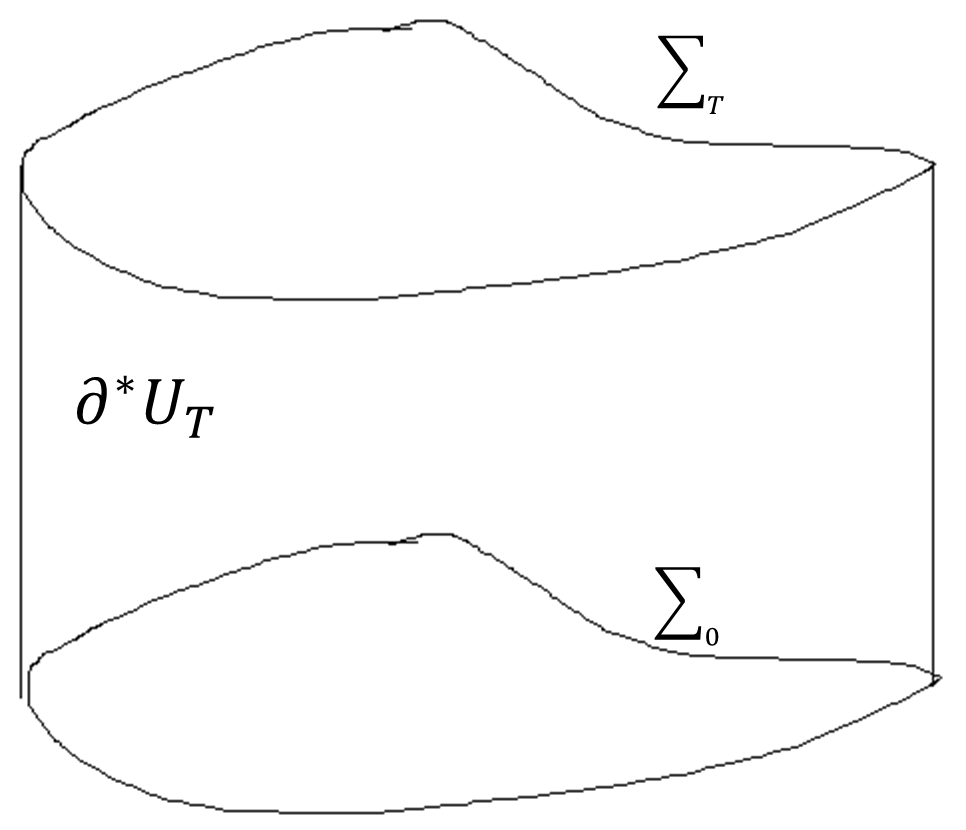
\includegraphics[scale=0.33]{9}
	\end{center}
\end{figure}
So $\pa U_T = \Sigma_0 \sqcup \Sigma_T \sqcup \pa^* U_T$. We define
\begin{align*}
Lu = -\sum_{i,j=1}^n (a^{ij}u_{x_i})_{x_j} + \sum_{i=1}^n b^i u_{x_i} + bu_t + cu
\end{align*}
where $a^{ij}, b^i, b,c \in C^1(\bar{U}_T)$. Further assume $a^{ij}$ satisfy the uniform ellipticity condition
\begin{align*}
\sum_{i,j=1}^n a^{ij}(x,t) \xi_i \xi_j \geq \theta |\xi|^2
\end{align*}
for some $\theta >0$, all $(x,t)\in U_T$, $\xi \in \reals^n$.

\quad The \textbf{initial-boundary value problem(IBVP)} we consider is:
\begin{align}
\begin{cases}
\begin{array}{ll}
u_{tt} + Lu = f & \text{in } U_T \\
u = \psi, \,\, u_t = \psi' & \text{on } \Sigma_0\\
u = 0 & \text{on } \pa^* U_T
\end{array}
\end{cases} \label{31}
\end{align}
e.g. The model in our mind is solving wave equation on a string given boundary conditions. If $L = - \Delta$, $f=0$, this is the wave equation on a bounded domain with specified initial conditions.
\s

As with the elliptic boundary value problem, we first find a weak formulation of the problem. Suppose $u\in C^2(\bar{U}_T)$ is a solution of (\ref{31}) and multiply the equation by $v\in C^2(\bar{U}_T)$ satisfying $v=0$ on $\pa^* U_T \cup \Sigma_T$. Then integrate over $U_T$.
\begin{align*}
\int_0^T dt \int_U dx (u_{tt} v + Luv) = \int_0^T dt \int_U dx fv
\end{align*}
Integrating by parts, we find
\begin{align}
\int_{U_T} \Big( -u_t v_t + \sum_{i,j} a^{ij}u_{x_i} v_{x_j} + \sum_i b^i u_{x_i} v + bu_t v  + cuv \Big) dxdt - \int_{\Sigma_0} \psi' v dx = \int_{U_T} fv dx dt \label{32}
\end{align}
Conversely, if (\ref{32}) holds for all $v\in C^2(\bar{U}_T)$ which vanish on $\Sigma_T \cup \pa^* U_T$ and $u\in C^2(\bar{U}_T)$ satisfies $u= \psi$ on $\Sigma_0$, $u=0$ on $\pa^* U_T$, undoing the integration by parts gives
\begin{align*}
\int_{U_T} (u_{tt}v + Lv - fv) dxdt + \int_{\Sigma_0} (u_t - \psi') vdx =0
\end{align*}
Taking $v\in C_c^{\infty}(U_T)$, the $\Sigma_0$ term vanishes and we deduce $u_{tt} + Lu = f$ in $U_T$. This implies
\begin{align*}
\int_{\Sigma_0} (u_t - \psi') vdx =0 \quad \forall v \in C_c^{\infty}(\Sigma_0) \quad \Rightarrow \quad u_t = \psi'
\end{align*}
The expression (\ref{32}) makes sense if $u\in H^1(U_T)$, $v\in H^1(U_T)$. This motivates the definition :
\s

\defi Suppose $f\in L^2(U_T)$, $\psi \in H_0^1(\Sigma_0)$, $\psi \in L^2(\Sigma_0)$ and $a^{ij}, b^i, b, c \in C^1(\bar{U}_T)$ with $a^{ij}$ satisfying uniform ellipticity condition in $U_T$. We say $u\in H^1(U_T)$ is a weak solution of the IBVP (\ref{31}) if
\begin{align*}
\begin{cases}
\begin{array}{lll}
u = \psi & \text{on } \Sigma_0 & \quad \text{ in the trace sense} \\
u = 0 & \text{on } \pa^* U_T & \quad \text{ in the trace sense}
\end{array}
\end{cases}
\end{align*}
and (\ref{32}) holds for all $v\in H^1(U_T)$ with $v=0$ on $\Sigma_T \cup \pa^* U_T$ in the trace class.
\s

Note that, we could not say $\pa_t u = \psi'$ on $\Sigma_0$ in trace sense, because $\pa_t u$ is just a $L^2$-function while we do not have trace theorem for $L^2$ functions.
\s

We cannot use Lax-Milgrim theorem as it is. But we can do something different to show unique existence of the solution in a different way.
\s

\thm A weak solution to (\ref{31}), if it exists, is unique.
\s

\textbf{Motivation :} Suppose we consider the standard wave equation
\begin{align*}
u_{tt}  - \Delta u = 0 \quad \text{in } U_T
\end{align*}
with the initial and boundary conditions as in (\ref{31}). Assume $u\in C^2(U_T)$. To show the solution is unique, sufficient to consider $\psi= \psi' =0$. Multiply by $u_t$ and integrate over $x\in U$.
\begin{align*}
\int_U u_{tt} u_t - \Delta u \cdot u_t dx =  \int_U u_{tt} u_t + Du \cdot Du_t dx = \frac{d}{dt} \int_U \frac{1}{2} u_t^2 + \frac{1}{2} |Du|^2 dx
\end{align*}
So if $u=u_t =0$ initially, then 
\begin{align*}
\int_{\Sigma_t} \frac{1}{2} u_t^2 + |Du|^2 dx =0 \quad \forall t\in (0,T)
\end{align*}
and therefore $u=0$ in $U_T$.

\quad We work in the same spirit for the general case where $u \in H^1(U_T)$, but we have to be more careful when doing this.
\s

\begin{proof}
\textbf{proof of theorem)} Note that by linearity, sufficient to prove that if $\psi = 0$, $\psi'=0$, $f=0$ then $u=0$. We want to use $u_t$ as a test function but it is not regular enough (does not vanish on $\Sigma_T$). Take
\begin{align*}
v(x,y) = \int_t^T e^{-\lambda s} u(x,s) ds
\end{align*}
for $\lambda\in \reals$ we choose later. We find $v\in H^1(U_T)$, $v=0$ on $\pa^* U_T \cup \Sigma_T$ and $v_t = -e^{-\lambda t} u \in H^1(U_T)$. Putting this into (\ref{32}) with $\psi = \psi' =f=0$, we have
\begin{align*}
\int_{U_T} \Big[ u_t u e^{-\lambda t} - \sum_{i,j} a^{ij} v_{tx_i} v_{x_j} e^{\lambda t} + \sum_{i} b^i u_{x_i} v - bv^2 e^{\lambda t} + (c- 1)uv -   vv_t e^{\lambda t} \Big] dxdt = 0
\end{align*}
Rewriting,
\begin{align*}
\textbf{(A)} =& \int_{U_T} \Big[ \frac{d}{dt} \Big( \frac{1}{2}u^2 e^{-\lambda t} -\frac{1}{2} \sum_{i,j}a^{ij} v_{x_i}v_{x_j} e^{\lambda t} - \frac{1}{2}v^2 e^{\lambda t} \Big) \\
&+ \frac{\lambda}{2} \Big( u^2 e^{-\lambda t} + \frac{1}{2} \sum_{i,j} a^{ij}v_{x_i}v_{x_j} e^{\lambda t} + v^2 e^{\lambda t} \Big) \Big] dxdt \\
=& \int_{U_T} \Big[ \frac{1}{2} \sum_{i,j} \dot{a}^{ij} v_{x_i}v_{x_j} e^{\lambda t} - \sum_{i} b^i u_{x_i} v + bv^2 e^{\lambda t} -(c-1)uv \Big] dxdt = \textbf{(B)}
\end{align*}
and
\begin{align*}
\textbf{(A)} = & \int_{\Sigma_T} \frac{1}{2} u^2 e^{-\lambda T} dx + \int_{\Sigma_0} \Big( \frac{1}{2} \sum_{i,j} v_{x_i} v_{x_j}  + \frac{1}{2} v^2\Big) \\
& + \frac{\lambda}{2} \int_{U_T} \Big( u^2 e^{-\lambda t} + \frac{1}{2} \sum_{i,j} a^{ij} v_{x_i}v_{x_j} + v^2 e^{\lambda t} \Big) dxdt
\end{align*}
and (using AM-GM inequality and that $a,b,c$ are of $C^1$)
\begin{align*}
\textbf{(B)} \leq C \int_{U_T} u^2 e^{-\lambda t} + (\sum_{i,j} a^{ij} v_{x_i} v_{x_j} + v^2)e^{\lambda t} dxdt
\end{align*}
for some constant $C$ independent of $\lambda$. Putting these together and taking $\lambda$ large enough, we have
\begin{align*}
(\lambda -2C) \int_{U_T} u^2 e^{-\lambda t} + (\sum_{i,j} a^{ij}v_{x_i}v_{x_j} + v^2)e^{\lambda t} dxdt \leq 0
\end{align*}
With $\lambda -2C \geq 0$, we have $u\equiv 0$

\eop
\end{proof}













\end{document}